\documentclass[11pt]{article}
\usepackage{classTools}


\begin{document}



% To include a problems set header, use the psHeader command
\psHeader{3}{Wed Sept. 28, 2022 (11:59pm)}

\textbf{Your name: }

\textbf{Collaborators: }

\textbf{No. of late days used on previous psets: }

\textbf{No. of late days used after including this pset: }


The purpose of this problem set is to solidify your understanding of the RAM model (and variants), and the relations between the RAM model, the Word-RAM model, Python programs, and variants. In particular, you will build skills in simulating one computational model by another and in evaluating the runtime of the simulations (both in theory and in practice).

\begin{enumerate}
 
    \item (Simulation in practice: RAMs on Python)  
    In the Github repository, we have given you a partially written Python implementation of a RAM Model simulator.  Your task is to fill in the missing parts of the code to obtain a complete RAM simulator.
     Your simulator should take as input a RAM Program $P$ and an input $x$, and simulate the execution of $P$ on $x$, and return whatever output $P$ produces (if it halts).  The RAM Program $P$ is given as a Python list $[v,C_0,C_1,\ldots,C_{\ell-1}]$, where $v$ is the number of variables used by $P$.  For simplicity, we assume that the variables are named $0,\ldots,v-1$ (rather than having names like ``tmpptr'' and ``insertvalue''), but you can introduce constants to give names to the variables.  The $0$\textsuperscript{th} variable will always be $\inputlen$, the $1$\textsuperscript{st} variable $\outputpointer$, and the $2$\textsuperscript{nd} variable $\outputlen$.  A command $C$ is given in the form of a list of the form $[\cmd]$, $[\cmd,i]$, $[\cmd,i,j]$, or $[\cmd,i,j,k]$, where $\cmd$ is the name of the command and $i,j,k$ are the indices of the variables or line numbers used in the command.  For example,  the command $\var_i = M[\var_j]$ would be represented as $(\READ,i,j)$.  See the Github repository for the precise syntax as well as some RAM programs you can use to test your simulator.

    \item (Empirically evaluating simulation runtimes and explaining them theoretically)  


Consider the following two RAM programs:

\begin{algorithm}[H]
\Input{A single natural number $N$ (as an array of length 1)}
\Output{$11^{2^N+1}$ (as an array of length 1)}
\Variables{$\inputlen, \outputpointer, \outputlen, \counter, \result$}
\setcounter{AlgoLine}{-1}
$\zero = 0$\;
$\one = 1$\;
$\eleven = 11$\;
$\outputlen = 1$\;
$\outputpointer = 0$\;
$\result = 11$\;
$\counter = M[\zero]$\;
\Indp
 IF $\counter == 0$ GOTO 11\;
$\result = \result * \result$\;
$\counter = \counter - \one$\;
IF $\zero == 0$ GOTO 7\;
\Indm
$\result = \result * \eleven$\; \label{line:done}
$M[\outputpointer]=\result$\;
\end{algorithm}


\begin{algorithm}[H]
\Input{A single natural number $N$ (as an array of length 1)}
\Output{$11^{2^N+1} \bmod 2^{32}$ (as an array of length 1)}
\Variables{$\inputlen, \outputpointer, \outputlen, \counter, \result, \temp, \W$}
\setcounter{AlgoLine}{-1}
$\zero = 0$\;
$\one = 1$\;
$\eleven = 11$\;
$\outputlen = 1$\;
$\outputpointer = 0$\;
$\result = 11$\;
$\W = 2^{32}$\;
$\counter = M[\zero]$\;
\Indp
IF $\counter == 0$ GOTO 15 \;
$\result = \result * \result$\;
$\temp = \result / \W$\;
$\temp = \temp \times \W$\;
$\result = \result - \temp$\;
$\counter = \counter - \one$\;
IF $\zero == 0$ GOTO 8 \;
\Indm
$\result = \result * \eleven$\;
\label{line:done2}
$\temp = \result / \W$\;
$\temp = \temp \times \W$\;
$\result = \result - \temp$\;
$M[\outputpointer]=\result$\; 
\end{algorithm}


\begin{enumerate}
    \item \label{itm:RAMtime} Exactly calculate (without asymptotic notation) the RAM-model running times of the above algorithms as a function of $N$.
    Which one is faster? 

\begin{proof}
Every line in RAM code takes constant time to implement here; in particular, the number of commands executed is the running time (this was clearly defined in class).

For the first program, the first seven commands are executed once each. Then lines 7-10 occur in a loop $N$ times, where $N$ is the input. At the end, line 7 is computed one more time to escape the loop, and then lines 11-12 are executed once each. In the end this means that $\Time_{prog_1} (N) = 4N + 10$.

For the second program, the first eight commands are executed once each. Then lines 8-14 occur in a loop $N$ times, where $N$ is the input. At the end, line 8 is computed one more time to escape the loop, and then lines 15-19 are executed once each. In the end this means that $\Time_{prog_1} (N) = 7N + 14$.
\end{proof}
    
    \item \label{itm:realtime} Using your RAM Simulator, run both RAM programs on inputs $N=0,1,2,\ldots,15$ and graph the actual running times (in clock time, not RAM steps).  (We have provided you with some timing and graphing code in the Github repository.) Which one is faster? 
    
\begin{proof}[Solution]
Here is the plot.
\\
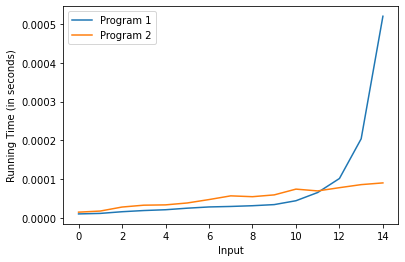
\includegraphics[width=5in]{2-2}

It looks like the first program is slightly faster until $N = 12$, at which point it becomes dramatically slower than the second program.
\end{proof}  
    
    \item Explain the discrepancies you see between Parts~\ref{itm:RAMtime} and \ref{itm:realtime}.  (Hint: What do we know about the relationship between the RAM and Word-RAM models, and why is it relevant to how efficiently the Python simulation runs?)  
    
\begin{proof}
We compute runtime theoretically by assuming that every single step in the RAM model has an equivalent length. However, this is not a good assumption when numbers get large. In particular, the Word-RAM model is useful because data cannot get infinitely big in programs; instead, there is a limitation on the size of a ``word", or any number we store. So it looks like the second program still runs on $O(n)$ time because its values are limited to being less than $2^{32}$; however, numbers in the first program get arbitrarily large, so they in fact become represented in ``bignum" notation, as discussed in class. Bignum notation makes multiplication of very large numbers possible, but it becomes much slower - if you have two blocks of numbers to multiply against each other, there are suddenly four multiplications to do, and the inputs reach a size where the are considerably more inputs than that, which is when the runtime for the first program becomes very large.
\end{proof}
    
    \item (optional\footnote{This problem won't make a difference between N, L, R-, and R grades.}) Give a theoretical explanation (using asymptotic estimates) of the shapes of the runtime curves you see in Part~\ref{itm:realtime}. You may need to do some research online and/or make guesses about how Python operations are implemented to come up with your estimates. 
    
\begin{proof}
It seems pretty clear that the runtime of the second program is $O(N)$ - the data bears this out in the size that we're given, and we can do additional tests to see that this holds for much larger values of $N$. 

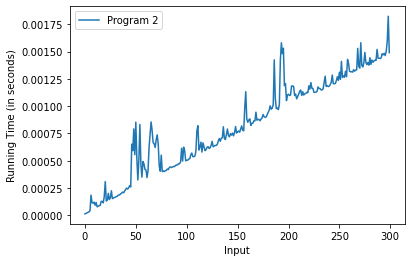
\includegraphics[width=5in]{2-3}

This makes logical sense - because the ``word size" of our numbers in this operation is kept to a minimum, there is no factor which would cause the program's runtime to change as $N$ increases.

The runtime of the first program becomes dominated by the multiplication lines as $N$ becomes large; in particular, this is line 9. We do this very large multiplication $N$ times, and a Google search reveals through the wisdom of some StackOverflow poster that for big numbers, multiplication is done with the Karatsuba algorithm, which has a runtime of around $O(n^{1.585})$ for multiplying two $n$-digit numbers, which is what we are doing. Now for some value of $N$, the number we are squaring in this algorithm has $\log_{10} 11^{2^{N - 1}} = 2^{N - 1} \log_{10} 11$ digits. Removing the constant, we find that the runtime for the first program is most easily represented as $O(2^{1.585(N - 1)})$.
\end{proof}

\end{enumerate}

\item (Simulating Word-RAM by RAM)  Show that for every Word-RAM program $P$, there is a RAM program $P'$ such that $P'$ halts on $x$ iff $P$ halts on $x$, and if they halt, then  $P'(x)=P(x)$ and 
       $$\Time_{P'}(x) = O\left(\Time_P(x)+n+w_0\right),$$
where $n$ is the length of $x$ and $w_0$ is the initial word size of $P$ on input $x$.  (This was stated without proof in Lecture Notes 7.) 

Your proof should use an {\em implementation-level} description, similar to our proof that RAM programs can be simulated by ones with at most $c$ registers.  Recall that Word-RAM programs have read-only variables $\memsize$ and $\wordlen$; you may want to start your simulation by calculating these variables as well as another variable representing $2^{\wordlen}$.  Then think about how each operation of a Word-RAM program $P$ can be simulated in a RAM program $P'$, taking care of any differences between their semantics in the Word-RAM model vs. the RAM model. Don't forget MALLOC!

\begin{proof}
First, we initialize the inputs. In a RAM program, we encode the input $x$ of length $n$ in the first $n$ memory locations (while everything else in memory is set to zero). Then we calculate a variable \inputlen which is the length of our input. It doesn't matter if we do this during input into memory or not; either way, we have to traverse the list once to find this information by adding to a counter, which is done in $n$ steps; in this process, every single input encountered takes 2 lines, so this requires $2n$ commands. This is where \memsize is calculated, and this process takes $O(n)$ time.

We also traverse the list once to find the largest entry of the list (we can do this by using a subtraction comparison test - if the current entry subtracted from our previous high is zero, we know that the result was clamped and we make our new high the current entry). We do a maximum of 3 lines in this process - subtracting the result, using a GOTO to see if the result is zero, and assigning a new high if so. In all, traversing the list takes a maximum of $3n$ commands. Then at the end, we divide the high value by 2 until we get 0; the number of times that we do this ends up being $\wordlen = w_0$. After that, we calculate $\maxval = 2^{\wordlen}$ (this can be done logarithmically in $O(\log \wordlen)$ time, but at worst takes $O(\wordlen)$ times). So in all this process takes $O(\wordlen)$ time.

Now we examine the execution of the program. The options for lines in execution are the same in both programs:

\begin{enumerate}
\item Assignment to a constant. In a Word-RAM program, we simply do not assign the variable to a constant if the constant is larger than \maxval, and we assign it normally otherwise. This means that in our RAM program, we require three lines to do this instead of one - the first line would subtract our constant from \maxval, the second line would institute a GOTO condition based on the result of the first line (i.e. we only assign the constant if it is less than \maxval) and the third would assign the constant if our condition is met.

\item Addition is clamped at \maxval. We use five lines to compute addition - in the first line, we subtract one addend from \maxval. In the second, we subtract the other. In the third, we use GOTO to check whether the result is zero. If so, we return \maxval (because the sum of our addition is greater than the maximum value); otherwise, return the sum of the two numbers.

\item Subtraction is implemented identically to the Word-RAM program, because we do not worry about our result getting too large.

\item Multiplication is defined identically to addition - we need five lines again. In this case, we use two lines to divide \maxval by the multiplicands. If the result is zero, we return $\maxval$ again; otherwise, we carry out the addition. This is to keep our values clamped.

\item Division is implemented identically to the Word-RAM program, because we do not worry about our result getting too large.

\item Reading from memory happens identically to the Word-RAM program, because all values area already clamped.

\item Writing to memory doesn't require a check on size, because we have already guaranteed that all variables are of appropriate word length by this point. This is a step where we might need the functionality of MALLOC, so I'll discuss it here. If we have filled the memory $M$ completely, we need to increment it (and $S$). We can do this by checking if the index of the memory compartment we are searching for exceeds the value of $S$ (subtraction test plus GOTO with zero bound); if so, we increment $S$ by 1, set $M[S - 1] = 0$ and change $S, \maxval, \wordlen$ if $S = \maxval$. These changes happen by adding one to \wordlen, multiplying \maxval by two, and doing the same for $S$. So in the end, this is a constant multiple of steps at the worst case.

\item GOTO. This is done exactly the same way as in the Word-RAM model, because we don't have to worry about memory or values getting too large.
\end{enumerate}

At the end of all this, no step takes more than a constant multiple of $O(\Time_P (x))$ time to implement. 

At the end of all of this, we examine the process of returning the output. Note that the output of our RAM and Word-RAM programs is always identical. Therefore by the time we reach this step, we already have the output lined up in the memory with existing values of \texttt{output\_len} and \texttt{output\_ptr}. Therefore we output the data the same way and we are done. We take $O(\Time_P (x))$ time to do this.

Adding everything together in the end, it is clear that our different steps added together reveal that 

$$\Time_{P'}(x) = O\left(\Time_P(x)+n+w_0\right),$$

as we desired. So we are done.
\end{proof}

\end{enumerate}


\end{document}
